\documentclass{article}\usepackage[]{graphicx}\usepackage[]{xcolor}
% maxwidth is the original width if it is less than linewidth
% otherwise use linewidth (to make sure the graphics do not exceed the margin)
\makeatletter
\def\maxwidth{ %
  \ifdim\Gin@nat@width>\linewidth
    \linewidth
  \else
    \Gin@nat@width
  \fi
}
\makeatother

\definecolor{fgcolor}{rgb}{0.345, 0.345, 0.345}
\newcommand{\hlnum}[1]{\textcolor[rgb]{0.686,0.059,0.569}{#1}}%
\newcommand{\hlsng}[1]{\textcolor[rgb]{0.192,0.494,0.8}{#1}}%
\newcommand{\hlcom}[1]{\textcolor[rgb]{0.678,0.584,0.686}{\textit{#1}}}%
\newcommand{\hlopt}[1]{\textcolor[rgb]{0,0,0}{#1}}%
\newcommand{\hldef}[1]{\textcolor[rgb]{0.345,0.345,0.345}{#1}}%
\newcommand{\hlkwa}[1]{\textcolor[rgb]{0.161,0.373,0.58}{\textbf{#1}}}%
\newcommand{\hlkwb}[1]{\textcolor[rgb]{0.69,0.353,0.396}{#1}}%
\newcommand{\hlkwc}[1]{\textcolor[rgb]{0.333,0.667,0.333}{#1}}%
\newcommand{\hlkwd}[1]{\textcolor[rgb]{0.737,0.353,0.396}{\textbf{#1}}}%
\let\hlipl\hlkwb

\usepackage{framed}
\makeatletter
\newenvironment{kframe}{%
 \def\at@end@of@kframe{}%
 \ifinner\ifhmode%
  \def\at@end@of@kframe{\end{minipage}}%
  \begin{minipage}{\columnwidth}%
 \fi\fi%
 \def\FrameCommand##1{\hskip\@totalleftmargin \hskip-\fboxsep
 \colorbox{shadecolor}{##1}\hskip-\fboxsep
     % There is no \\@totalrightmargin, so:
     \hskip-\linewidth \hskip-\@totalleftmargin \hskip\columnwidth}%
 \MakeFramed {\advance\hsize-\width
   \@totalleftmargin\z@ \linewidth\hsize
   \@setminipage}}%
 {\par\unskip\endMakeFramed%
 \at@end@of@kframe}
\makeatother

\definecolor{shadecolor}{rgb}{.97, .97, .97}
\definecolor{messagecolor}{rgb}{0, 0, 0}
\definecolor{warningcolor}{rgb}{1, 0, 1}
\definecolor{errorcolor}{rgb}{1, 0, 0}
\newenvironment{knitrout}{}{} % an empty environment to be redefined in TeX

\usepackage{alltt}
\usepackage{amsmath} %This allows me to use the align functionality.
                     %If you find yourself trying to replicate
                     %something you found online, ensure you're
                     %loading the necessary packages!
\usepackage{amsfonts}%Math font
\usepackage{graphicx}%For including graphics
\usepackage{hyperref}%For Hyperlinks
\usepackage[shortlabels]{enumitem}% For enumerated lists with labels specified
                                  % We had to run tlmgr_install("enumitem") in R
\hypersetup{colorlinks = true,citecolor=black} %set citations to have black (not green) color
\usepackage{natbib}        %For the bibliography
\setlength{\bibsep}{0pt plus 0.3ex}
\bibliographystyle{apalike}%For the bibliography
\usepackage[margin=0.50in]{geometry}
\usepackage{float}
\usepackage{multicol}

%fix for figures
\usepackage{caption}
\newenvironment{Figure}
  {\par\medskip\noindent\minipage{\linewidth}}
  {\endminipage\par\medskip}
\IfFileExists{upquote.sty}{\usepackage{upquote}}{}
\begin{document}

\vspace{-1in}
\title{Lab 8 -- MATH 240 -- Computational Statistics}

\author{
  Avery Johnson \\
  Colgate University  \\
  Department of Mathematics  \\
  {\tt aqjohnson@colgate.edu}
}

\date{}

\maketitle

\begin{multicols}{2}
\begin{abstract}
The Beta distribution is a flexible probability distribution on $[0,1]$, commonly used for modeling proportions and probabilities. This lab examines how graphical and numerical summaries of Beta-distributed samples connect to the underlying population distribution, particularly as sample size increases. Two estimation methods, the Method of Moments (MOM) and Maximum Likelihood Estimation (MLE), are compared using death rate data. Results show that MLE provides more precise estimates for $\alpha$, demonstrating a slight advantage over MOM, although both yield similar results. 

\end{abstract}

\noindent \textbf{Keywords:} 
Beta distribution, moments, mean, variance, skewness, kurtosis, MOM estimator, MLE estimator.

\section{Introduction}
The Beta distribution is a continuous probability distribution defined on $[0,1]$, commonly used to model proportions, probabilities, and rates. Controlled by two parameters, $\alpha$ and $\beta$, its shape ranges from highly symmetric to highly skewed, making it flexible for various statistical applications. This lab investigates the properties of the Beta distribution, compares population and sample-based estimates, and applies parameter estimation techniques to real-world data. Additionally, the effectiveness of MOM and MLE in estimating $\alpha$ and $\beta$ is assessed through simulation.

\section{Density Functions and Parameters}
The probability density function (PDF) of a beta distribution is given by:
$$
f_X(x \mid \alpha, \beta) = \frac{\Gamma(\alpha + \beta)}{\Gamma \alpha \Gamma \beta} x^{\alpha-1} (1-x)^{\beta - 1} I(x \in [0,1])
$$
where $I(x \in [0,1]) = 1$ when $x \in [0, 1]$ and $0$ otherwise.

To visualize the impact of the parameters $\alpha$ and $\beta$ on the distribution, four cases were examined: \texttt{Beta(2,5)}, \texttt{Beta(5,5)}, \texttt{Beta(5,2)}, and \texttt{Beta(0.5,0.5)}. The first distribution is right-skewed, the second is symmetric, the third is left-skewed, and the forth is U-shaped. The plots in Figure \ref{populationfigures} demonstrate this, illustrating that increasing $\alpha$ shifts the distribution towards 1, while increasing $\beta$ shifts it towards zero. When $\alpha= \beta$, the distribution is symmetric.

\section{Properties}
Several important properties of the Beta distribution include the mean, variance, skewness, and excess kurtosis. These values were calculated for each Beta distribution using established mathematical formulas (Table \ref{populationsummary}). To verify accuracy, numerical integration was performed to compute moments directly from the PDF using a custom function, \texttt{beta.moment()}, which calculated both the centered and uncentered moments. The results aligned with theoretical expectations.

Random samples of size $n=500$ were generated from each Beta distribution. Histograms were plotted alongside the true PDFs in Figure \ref{samplehistograms}, and numerical summaries were computed (Table \ref{samplestatistics}). Comparing Table \ref{samplestatistics} with Table \ref{populationsummary}, along with analyzing Figure \ref{samplehistograms}, confirms that sample estimates closely approximate theoretical values.

To analyze sample size effects, cumulative statistics were plotted for the \texttt{Beta(2,5)} distribution using the \texttt{cumstats} package in \texttt{R} \citep{cumstats}. A single sample was first examined, followed by a simulation using a \texttt{for()} loop to generate data sets of size 500, adding new cumulative statistics lines at each iteration. The results (Figure \ref{cumstats} in the Appendix) show that variability is high for small samples but decreases as $n$ increases, illustrating convergence to population values. Results indicate the importance of sample size.



% latex table generated in R 4.4.2 by xtable 1.8-4 package
% Thu Mar 27 16:04:56 2025
\begin{table}[H]
\centering
\begingroup\small
\begin{tabular}{rrrrrr}
  \hline
alpha & beta & mean & var & skew & kurtosis \\ 
  \hline
2.00 & 5.00 & 0.29 & 0.03 & 0.60 & -0.12 \\ 
  5.00 & 5.00 & 0.50 & 0.02 & 0.00 & -0.46 \\ 
  5.00 & 2.00 & 0.71 & 0.03 & -0.60 & -0.12 \\ 
  0.50 & 0.50 & 0.50 & 0.12 & 0.00 & -1.50 \\ 
   \hline
\end{tabular}
\endgroup
\caption{Population-Level Summary} 
\label{populationsummary}
\end{table}


% latex table generated in R 4.4.2 by xtable 1.8-4 package
% Thu Mar 27 16:04:56 2025
\begin{table}[H]
\centering
\begingroup\small
\begin{tabular}{rrrrrr}
  \hline
alpha & beta & mean & var & skew & kurtosis \\ 
  \hline
2.00 & 5.00 & 0.29 & 0.03 & 0.57 & -0.23 \\ 
  5.00 & 5.00 & 0.50 & 0.02 & -0.06 & -0.58 \\ 
  5.00 & 2.00 & 0.71 & 0.03 & -0.57 & -0.23 \\ 
  0.50 & 0.50 & 0.51 & 0.13 & -0.02 & -1.51 \\ 
   \hline
\end{tabular}
\endgroup
\caption{Sample Summary} 
\label{samplestatistics}
\end{table}


\pagebreak
\section{Estimators}
Since the true value of $\alpha$ and $\beta$ are unknown in real-world applications, parameter estimation methods are essential. Two widely used techniques are the Method of Moments (MOM) and Maximum Likelihood Estimation (MLE). MOM estimates parameters by equating sample moments to their corresponding population moments. Using the \texttt{nleqslv} package in \texttt{R}, parameters were chosen to match sample and population moments. MLE is a more general and widely used technique for parameter estimation. It finds the values of $\alpha$ and $\beta$ that maximize the likelihood of the observed data. The likelihood function is a product of the Beta PDF evaluated at each data point, but computationally, it is easier to work with the log-likelihood function. The \texttt{optim()} function in \texttt{R} was used to maximize the log-likelihood. MLE is generally regarded as more efficient since it often provides more precise estimates.

\section{Death Rates Example}
The flexibility of the Beta distribution was tested by modeling real-world death rate data from the world bank \citep{deathrates}. The data, representing deaths per 1,000 citizens, was transformed into a rate and fitted to a Beta distribution using both MOM and MLE. Parameter estimates were obtained by solving moment equations for MOM and optimizing the likelihood function for MLE (Table \ref{momandmle}). While the estimates for $\alpha$ weere similar across methods, the estimates for $\beta$ differed slightly.


% latex table generated in R 4.4.2 by xtable 1.8-4 package
% Thu Mar 27 16:04:56 2025
\begin{table}[H]
\centering
\begingroup\small
\begin{tabular}{lrr}
  \hline
Method & Alpha & Beta \\ 
  \hline
MOM & 8.43 & 1003.46 \\ 
  MLE & 8.27 & 985.05 \\ 
   \hline
\end{tabular}
\endgroup
\caption{MOM and MLE Estimates} 
\label{momandmle}
\end{table}


To visualize the results, histograms of the empirical data were plotted with the estimated Beta distributions superimposed (Figure \ref{estimatedhistogram}). Both methods produced reasonable fits. To determine which estimators we should use, then, we computed bias, precision, and mean squared error (Table \ref{biasprecision}). Density plots (Figure \ref{densitycomparison}) further helped us visualize estimator differences. The results indicate that while MLE provided more narrow (precise) estimates for $\alpha$, both methods performed similarly overall.

\section{Conclusion}
This study illustrates the flexibility of the Beta distirbution and its usefulness in modeling proportion-based data. Graphical and numerical summaries show that sample estimates converge to population values as sample size increases. Additionally, the comparison of MOM and MLE estimators reveals that while both methods yield accurate and comparable results, MLE generally provides more precise parameter estimates. These findings reinforce the importance of selecting appropriate estimation techniques depending on the application and data characteristics.

\columnbreak

%%%%%%%%%%%%%%%%%%%%%%%%%%%%%%%%%%%%%%%%%%%%%%%%%%%%%%%%%%%%%%%%%%%%%%%%%%%%%%%%
% Bibliography
%%%%%%%%%%%%%%%%%%%%%%%%%%%%%%%%%%%%%%%%%%%%%%%%%%%%%%%%%%%%%%%%%%%%%%%%%%%%%%%%
\vspace{2em}

\begin{tiny}
\bibliography{bib}
\end{tiny}


\end{multicols}

%%%%%%%%%%%%%%%%%%%%%%%%%%%%%%%%%%%%%%%%%%%%%%%%%%%%%%%%%%%%%%%%%%%%%%%%%%%%%%%%
% Appendix
%%%%%%%%%%%%%%%%%%%%%%%%%%%%%%%%%%%%%%%%%%%%%%%%%%%%%%%%%%%%%%%%%%%%%%%%%%%%%%%%
\newpage
\onecolumn
\section{Appendix}

\subsection{Density Function and Parameters}
\subsubsection{Population Distribution Figures}
\begin{knitrout}\scriptsize
\definecolor{shadecolor}{rgb}{0.969, 0.969, 0.969}\color{fgcolor}
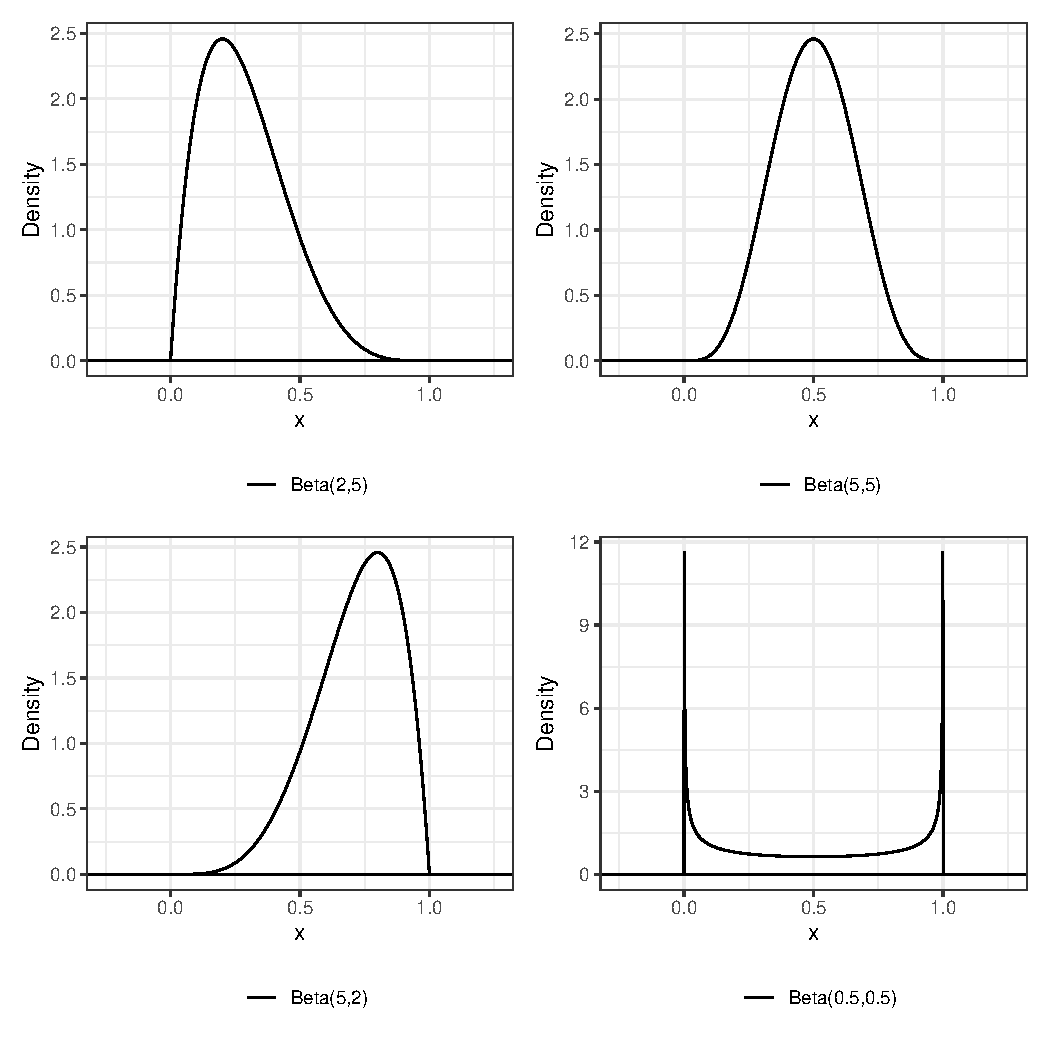
\includegraphics[width=\maxwidth]{figure/plot1-1} 
\end{knitrout}

\begin{figure}[H]
\begin{center}

\caption{Population Figures for Various Beta Distributions}
\label{populationfigures} %we can now reference plot1
\end{center}
\end{figure}

\pagebreak
\subsection{Properties}
\subsubsection{Sample Distribution Figures}
\begin{knitrout}\scriptsize
\definecolor{shadecolor}{rgb}{0.969, 0.969, 0.969}\color{fgcolor}
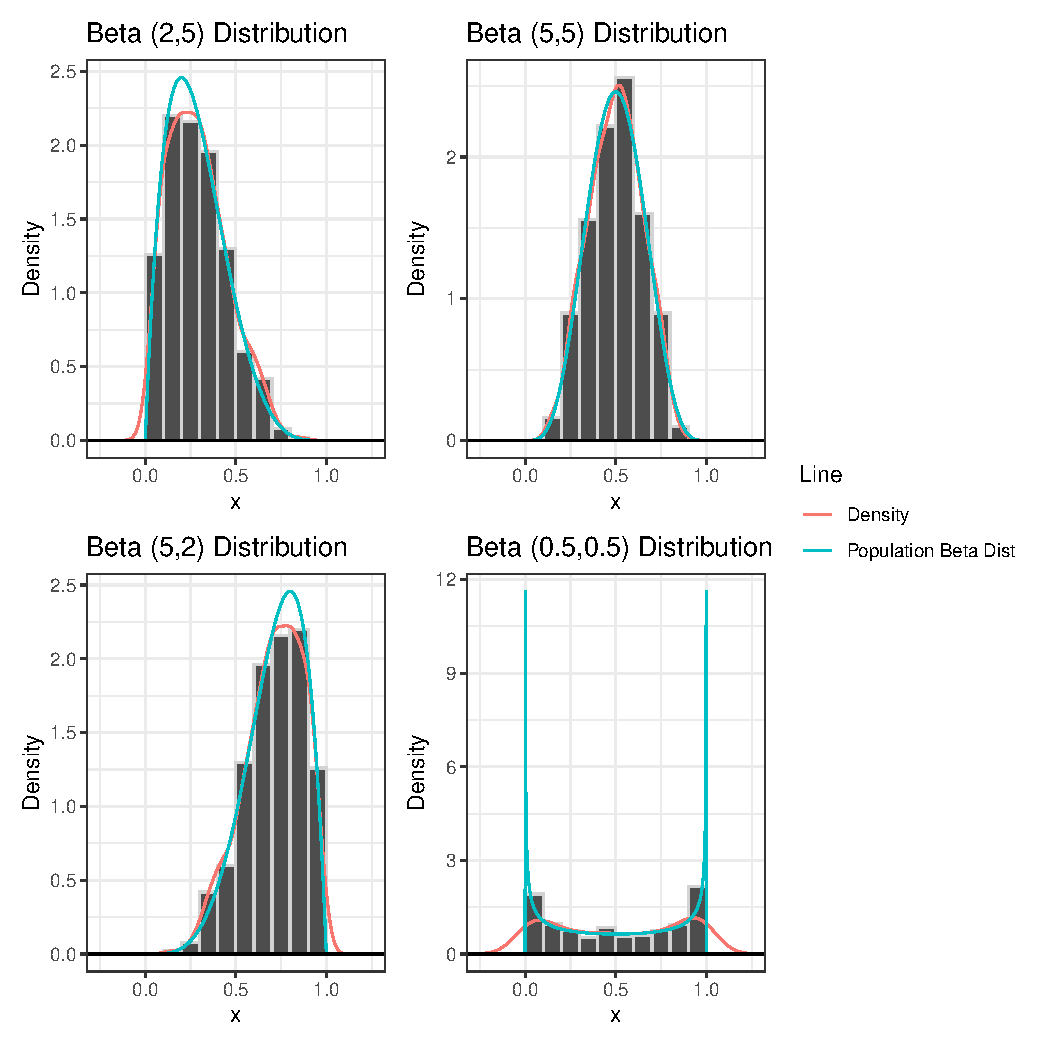
\includegraphics[width=\maxwidth]{figure/plot2-1} 
\end{knitrout}

\begin{figure}[H]
\begin{center}

\caption{Sample Figures for Various Beta Distributions}
\label{samplehistograms} %we can now reference plot1
\end{center}
\end{figure}

\pagebreak
\subsubsection{Cumulative Statistics: Does Sample Size Matter?}

\begin{knitrout}\scriptsize
\definecolor{shadecolor}{rgb}{0.969, 0.969, 0.969}\color{fgcolor}
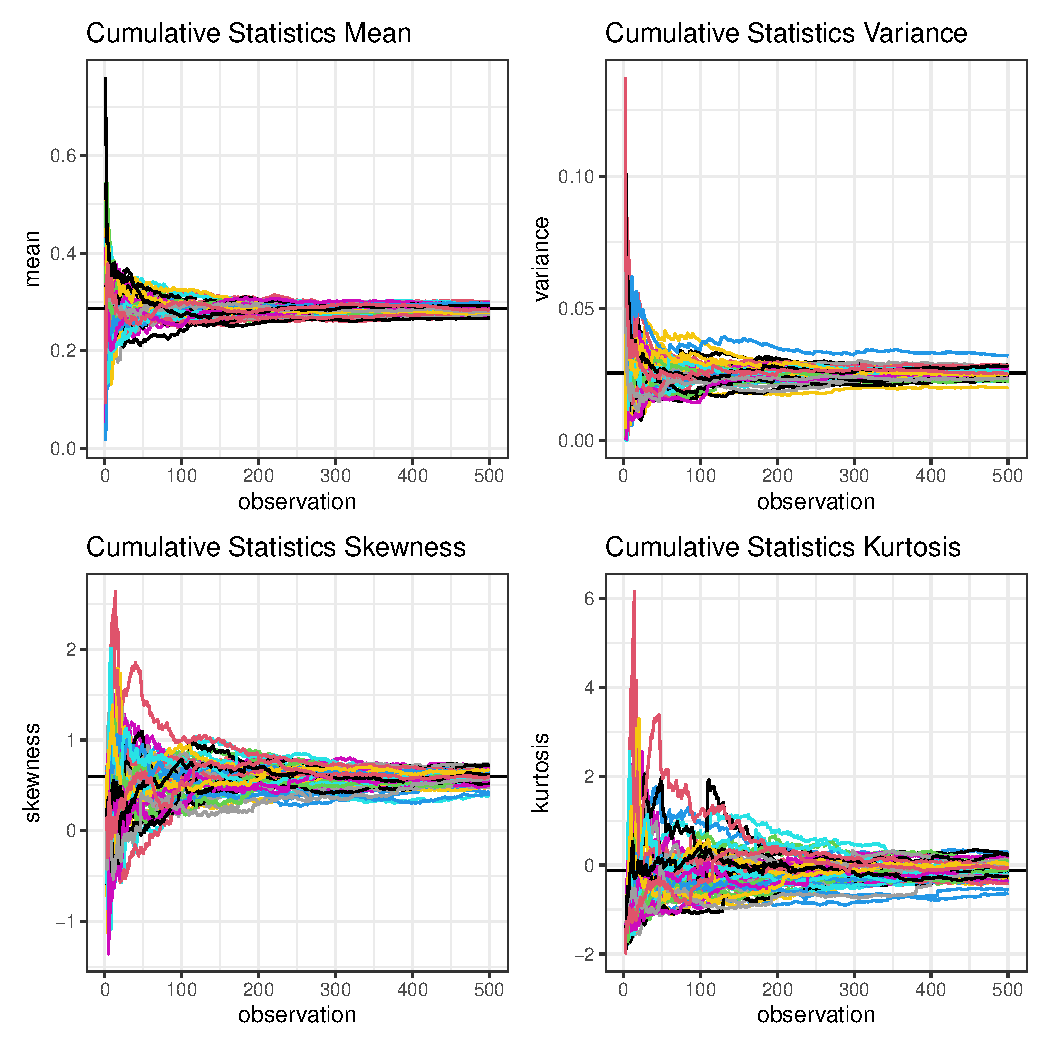
\includegraphics[width=\maxwidth]{figure/plot3-1} 
\end{knitrout}
\begin{figure}[H]
\begin{center}

\caption{Cumulative Statistics as Sample Size Increases}
\label{cumstats} %we can now reference plot1
\end{center}
\end{figure}

\pagebreak
\subsubsection{Modeling the Variation}
\begin{knitrout}\scriptsize
\definecolor{shadecolor}{rgb}{0.969, 0.969, 0.969}\color{fgcolor}
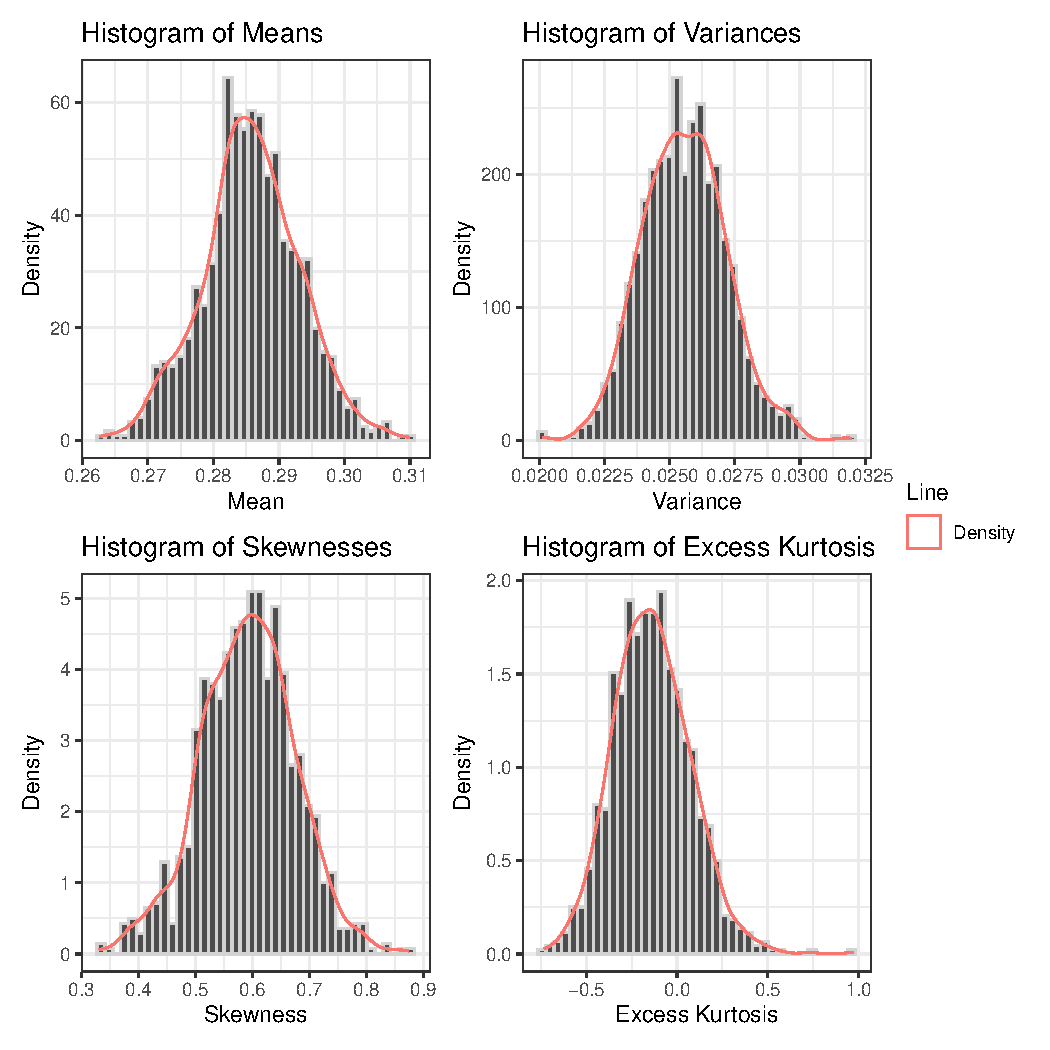
\includegraphics[width=\maxwidth]{figure/plot4-1} 
\end{knitrout}
\begin{figure}[H]
\begin{center}

\caption{Modeling the Variation of Statistics}
\label{variation} %we can now reference plot1
\end{center}
\end{figure}

\pagebreak
\subsection{Estimators}
\subsection{Example}
\subsubsection{MOM vs. MLE Estimates}
\begin{knitrout}\scriptsize
\definecolor{shadecolor}{rgb}{0.969, 0.969, 0.969}\color{fgcolor}
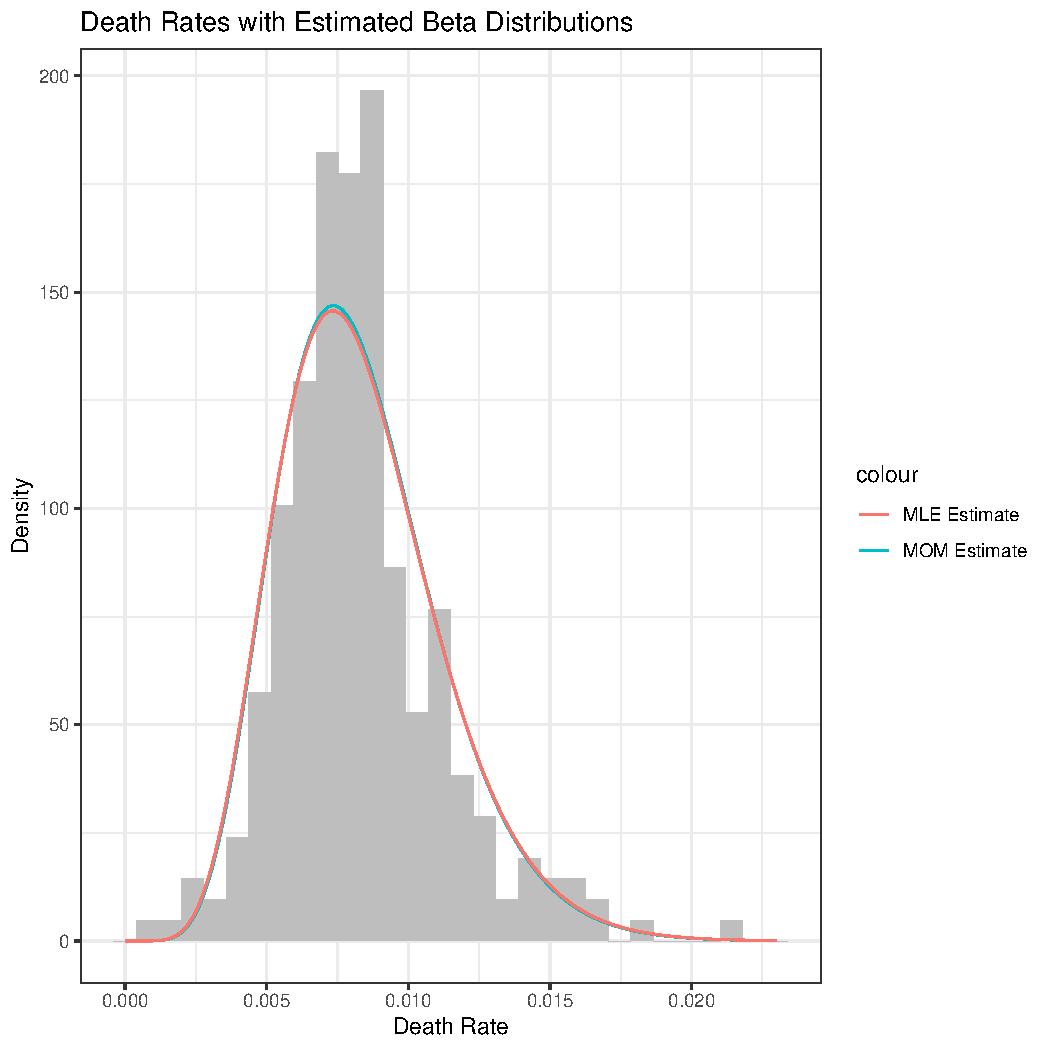
\includegraphics[width=\maxwidth]{figure/plot5-1} 
\end{knitrout}
\begin{figure}[H]
\begin{center}

\caption{Estimated Beta Distributions}
\label{estimatedhistogram} %we can now reference plot1
\end{center}
\end{figure}

\pagebreak

\subsubsection{Bias, Precision, and Mean Squared Error of Estimates}

% latex table generated in R 4.4.2 by xtable 1.8-4 package
% Thu Mar 27 16:05:26 2025
\begin{table}[H]
\centering
\begingroup\small
\begin{tabular}{lrrrrrr}
  \hline
Parameter & Bias\_MOM & Bias\_MLE & Precision\_MOM & Precision\_MLE & MSE\_MOM & MSE\_MLE \\ 
  \hline
Alpha & 0.08 & 0.07 & 1.83 & 2.13 & 0.55 & 0.48 \\ 
  Beta & 10.29 & 9.11 & 0.00 & 0.00 & 8288.46 & 7132.70 \\ 
   \hline
\end{tabular}
\endgroup
\caption{Bias, Precision, and Mean Squared Error} 
\label{biasprecision}
\end{table}


\pagebreak
\subsubsection{Estimated Density for MOM and MLE}
\begin{knitrout}\scriptsize
\definecolor{shadecolor}{rgb}{0.969, 0.969, 0.969}\color{fgcolor}
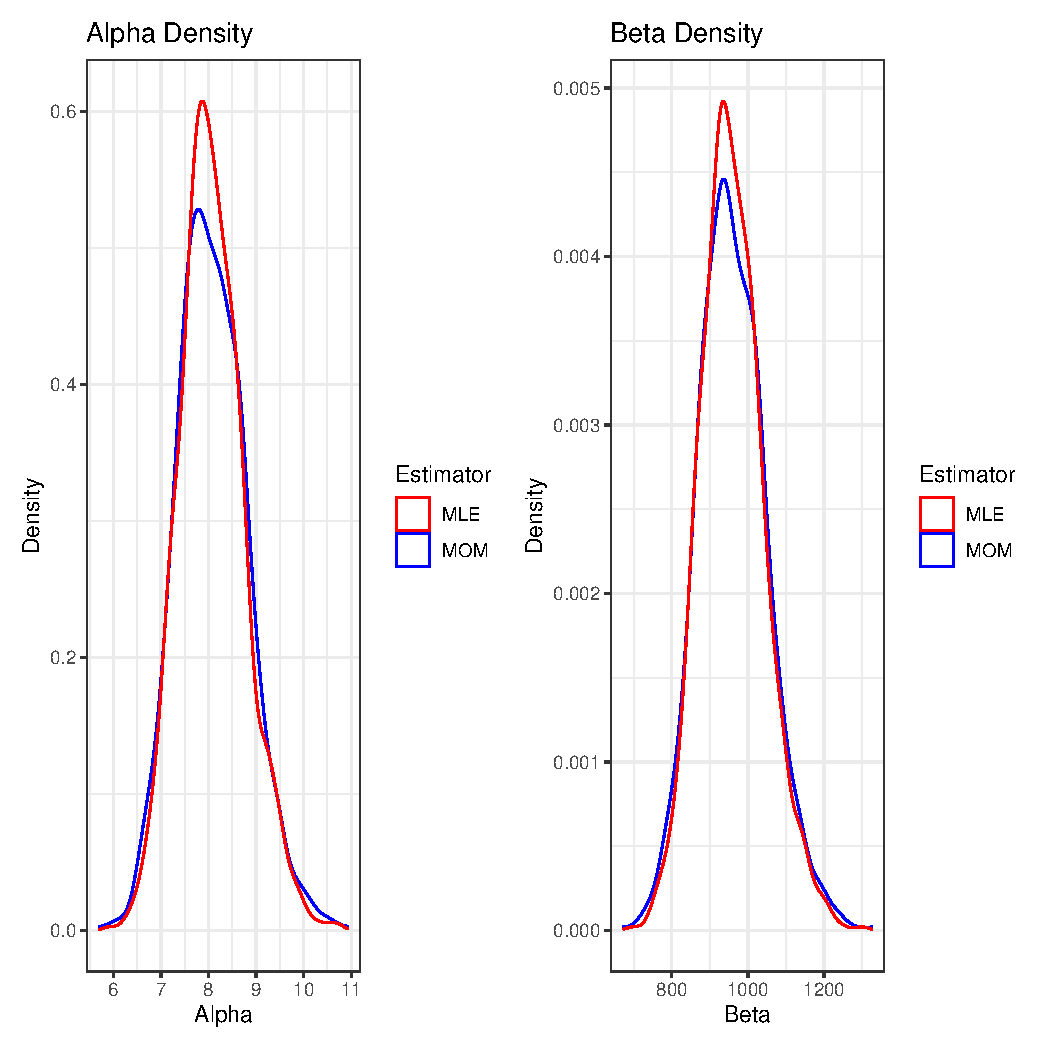
\includegraphics[width=\maxwidth]{figure/plot6-1} 
\end{knitrout}
\begin{figure}[H]
\begin{center}

\caption{Estimated Densities for MOM and MLE}
\label{densitycomparison} %we can now reference plot1
\end{center}
\end{figure}

\end{document}
